\chapter{Results}
\label{chap:results}


criticality - godiva, homogenized cube, single pin,  small array, large array
fixed source - water slab, accelerator driven subcritical?
compare w serpent and mcnp

collision estimator values are shown for serpent and mcnp (since this is what warp uses as well)

computer stats

define pcm

\begin{table}[h]
\centering
\caption{Summary of $k_\mathrm{eff}$ single-run results of the WARP benchmarks with 20/40 discarded/active criticality cycles and $10^5$ histories per cycle.}
\label{benchmark_summary}
\begin{tabular}{| l | r | r | r | r | r |}
 \hline
 Benchmark & MCNP 6.1 & Serpent 2.1.18 & WARP & $\Delta$ M & $\Delta$ S  \\
\hline
\hline
\multicolumn{6}{|l|}{Jezebel}  \\
\hline
 $k_\mathrm{eff}$ & 1.027509$\pm$0.0005 & 1.02748$\pm$0.00052 & 1.02789 & -38.1 pcm & -41 pcm  \\
 \hline
 Runtime               & 2.32 m & 9.50868 m & 0.2752 m & 8.4  & 34.6  \\
 \hline
 \hline
\multicolumn{6}{|l|}{Homogenized Block }\\
\hline
 $k_\mathrm{eff}$ & 0.943049$\pm$0.0003 & 0.940306$\pm$0.00046 & 0.941916 & 113 pcm & -161 pcm   \\
 \hline
 Runtime               &  25.58 m & 18.7190 m & 0.761 m & 33.6  & 24.6  \\
 \hline
  \hline
\multicolumn{6}{|l|}{Pin Cell}\\
\hline
 $k_\mathrm{eff}$ & 0.381435$\pm$0.0008 &  0.380511$\pm$0.00128 & 0.380586 & 84.9 pcm &  -7.5 pcm    \\
 \hline
 Runtime               & 55.85 m & 40.0035 m &  2.81583 m &  19.8 & 14.2  \\
 \hline
  \hline
\multicolumn{6}{|l|}{15-sided Hex Assembly}\\
\hline
 $k_\mathrm{eff}$ & 1.437465$\pm$0.0004 & 1.44704$\pm$0.00046 & 1.4442 & -673 pcm & 284 pcm  \\
 \hline
 Runtime               & 25.34 m &  26.3349 m &  3.2395 m  & 7.8 & 8.1  \\
 \hline
\end{tabular}
\end{table}


\begin{table}[h]
\centering
\caption{Summary of $k_\mathrm{eff}$ single-run results of the WARP benchmarks with 20/40 discarded/active criticality cycles and $10^6$ histories per cycle.}
\label{benchmark_summary}
\begin{tabular}{| l | r | r | r | r | r |}
 \hline
 Benchmark & MCNP 6.1 & Serpent 2.1.18 & WARP & $\Delta$ M & $\Delta$ S  \\
\hline
\hline
\multicolumn{6}{|l|}{Jezebel}  \\
\hline
 $k_\mathrm{eff}$ & 1.027957$\pm$0.0001 & $\pm$ &  &  &   \\
 \hline
 Runtime               & 22.79 m &  m &  m &   &   \\
 \hline
 \hline
\multicolumn{6}{|l|}{Homogenized Block }\\
\hline
 $k_\mathrm{eff}$ & &  &  & &    \\
 \hline
 Runtime               & m &  m &  m & &  \\
 \hline
  \hline
\multicolumn{6}{|l|}{Pin Cell}\\
\hline
 $k_\mathrm{eff}$ & &  &  & &    \\
 \hline
 Runtime               & m &  m &  m & &  \\
 \hline
  \hline
\multicolumn{6}{|l|}{15-sided Hex Assembly}\\
\hline
 $k_\mathrm{eff}$ & &  &  & &    \\
 \hline
 Runtime               & m &  m &  m & &  \\
 \hline
\end{tabular}
\end{table}

\begin{figure}[h!] 
\centering
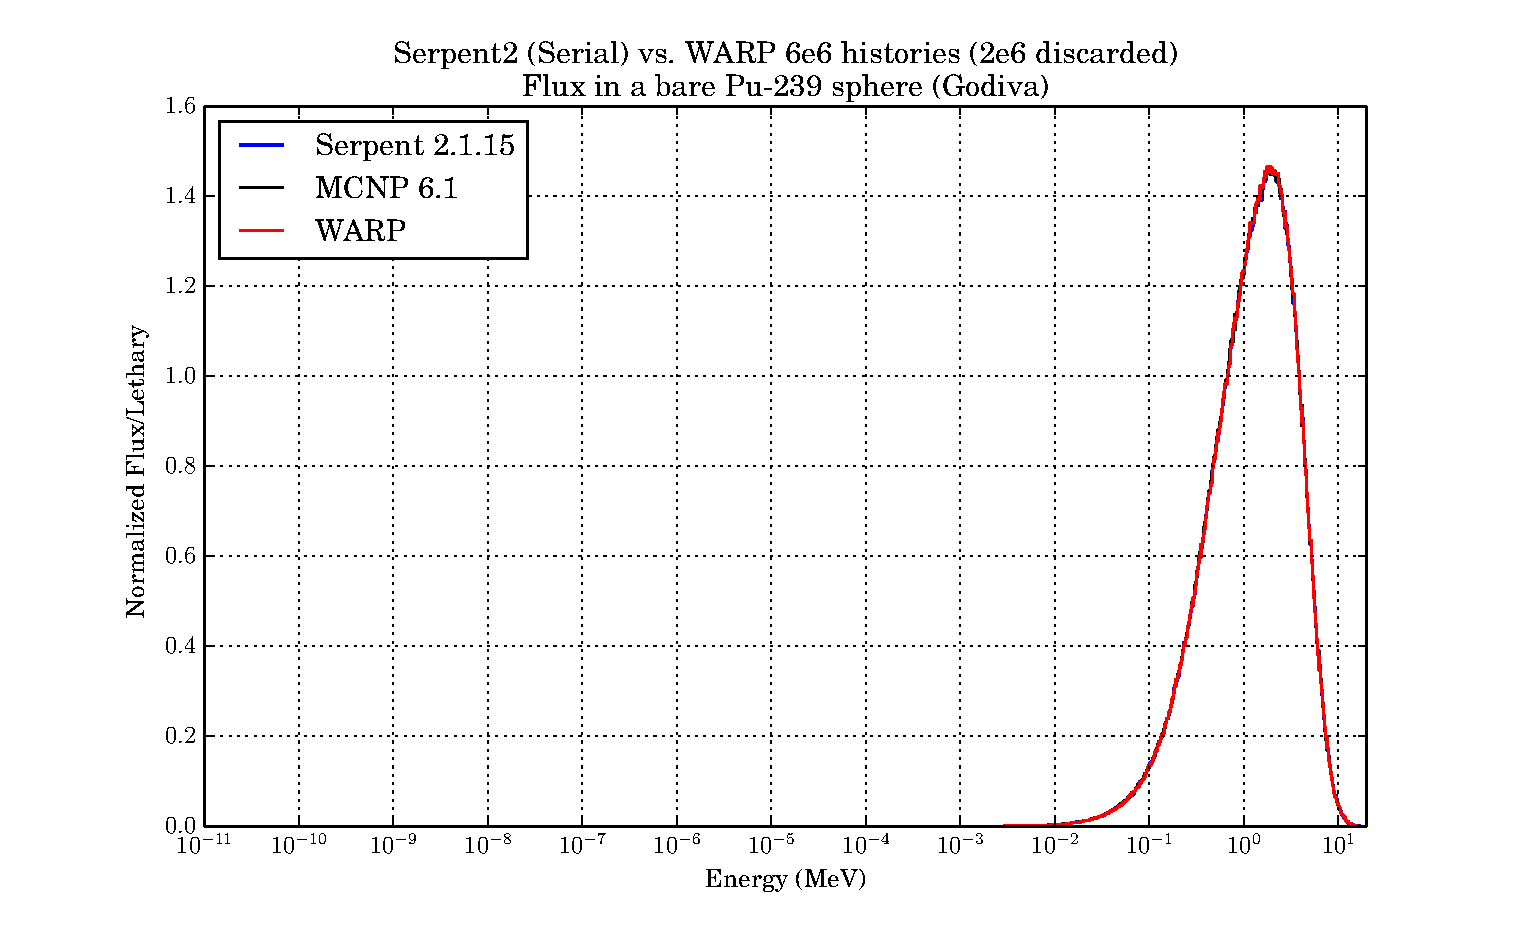
\includegraphics[width=0.8\textwidth]{graphics/finalresults/godiva_spec.eps}
\caption{Spectrum comparison in a ``godiva'' bare pu-239 sphere.. \label{godiva_spec} }
\end{figure}

\begin{figure}[h!] 
\centering
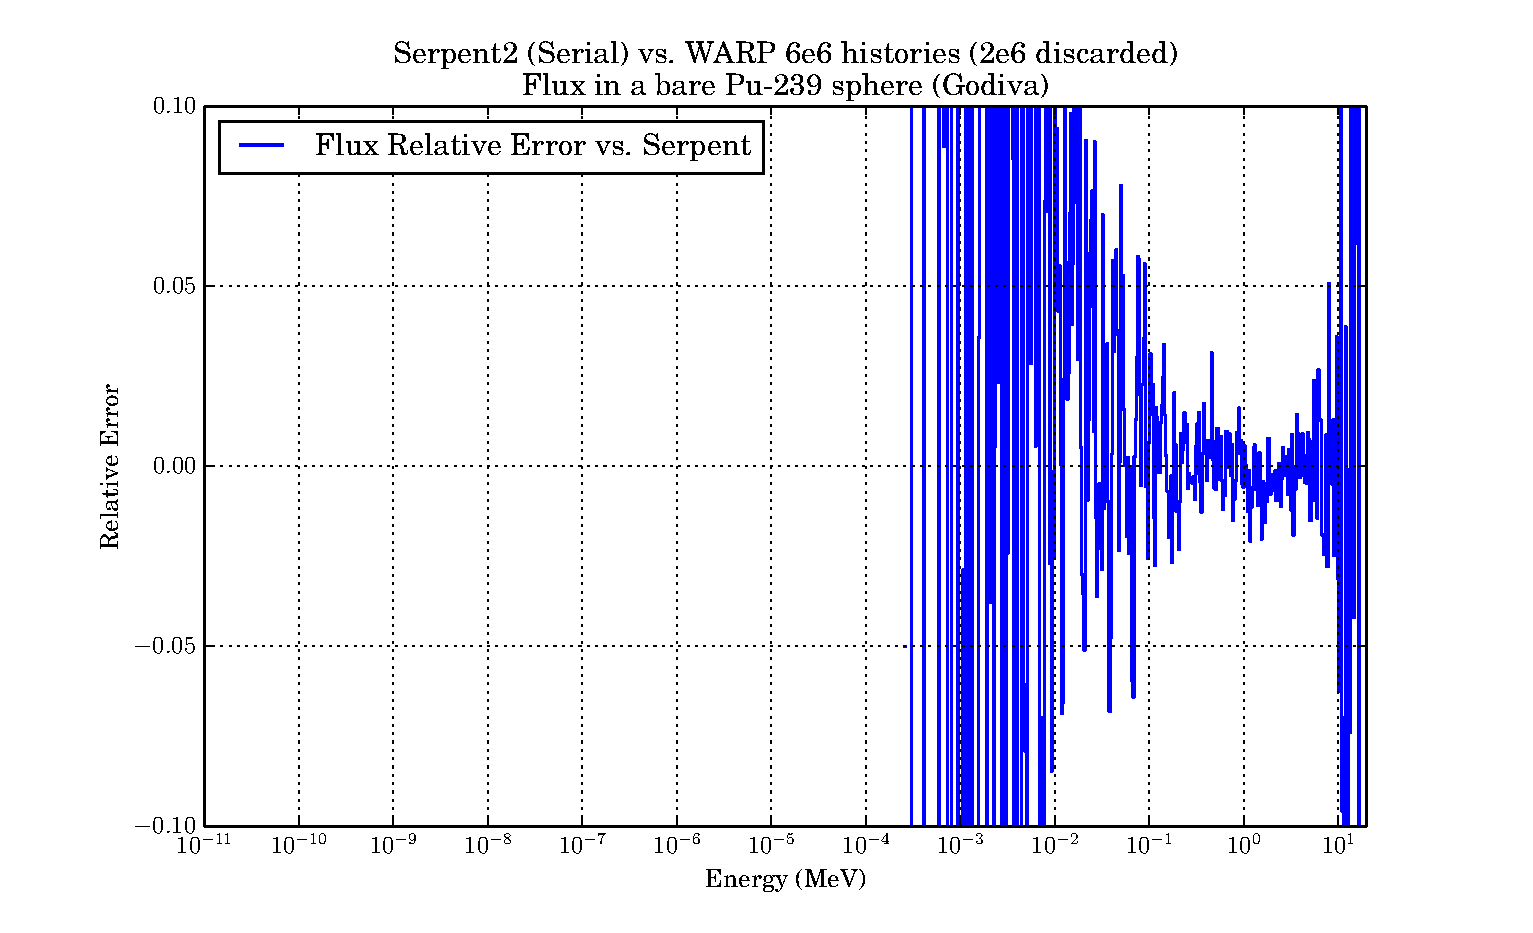
\includegraphics[width=0.8\textwidth]{graphics/finalresults/godiva_spec_err.eps}
\caption{Error of the spectrum calculated by WARP relative to that of Serpent in a ``godiva'' bare pu-239 sphere.. \label{godiva_spec_err} }
\end{figure}

\begin{figure}[h!]
\centering
\begin{subfigure}{.5\textwidth}
  \centering
  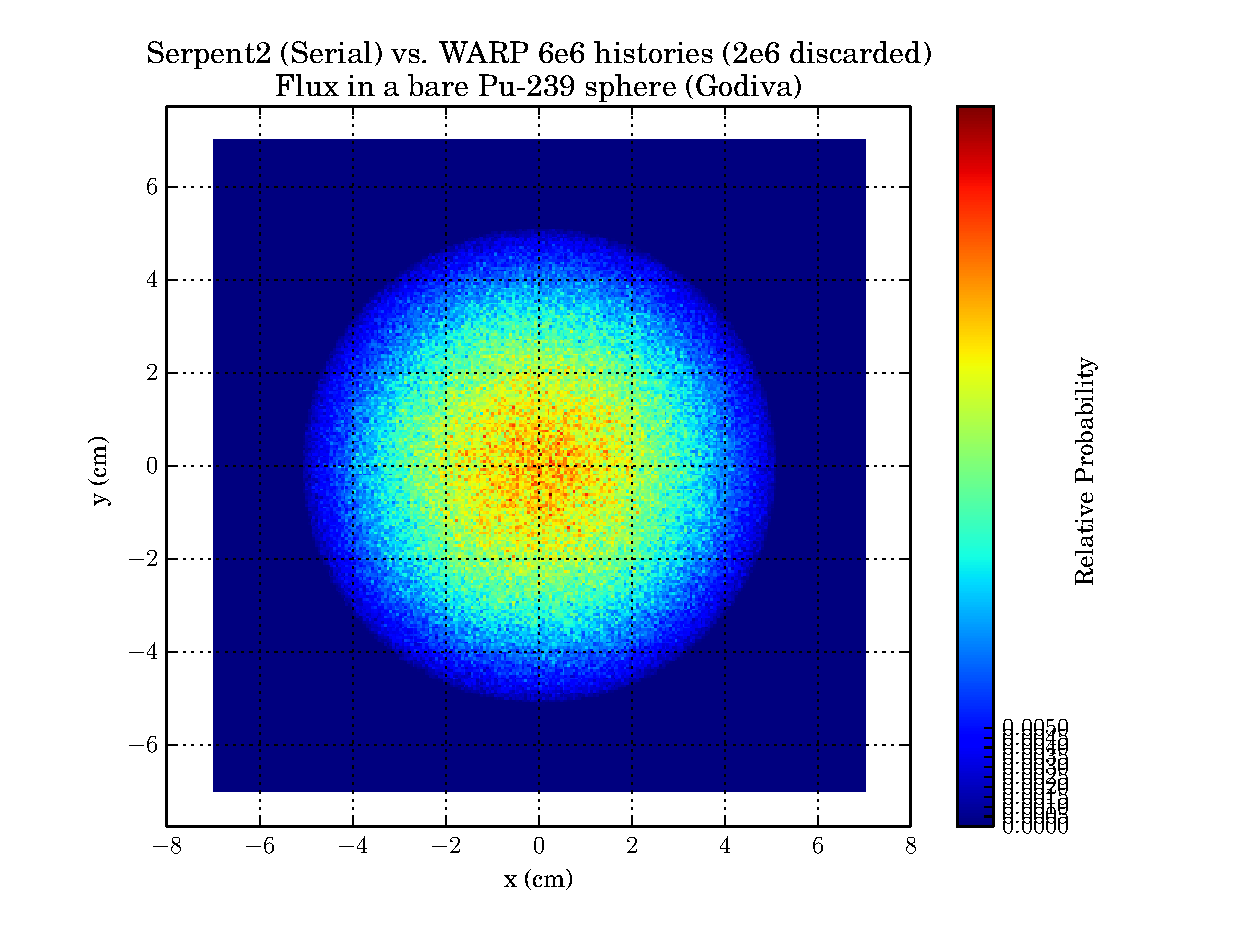
\includegraphics[width=\linewidth]{graphics/finalresults/godiva_fiss1.eps}
  \caption{$x-y$ slice, $z$ collapsed}
  \label{fig:sub1}
\end{subfigure}%
\begin{subfigure}{.5\textwidth}
  \centering
  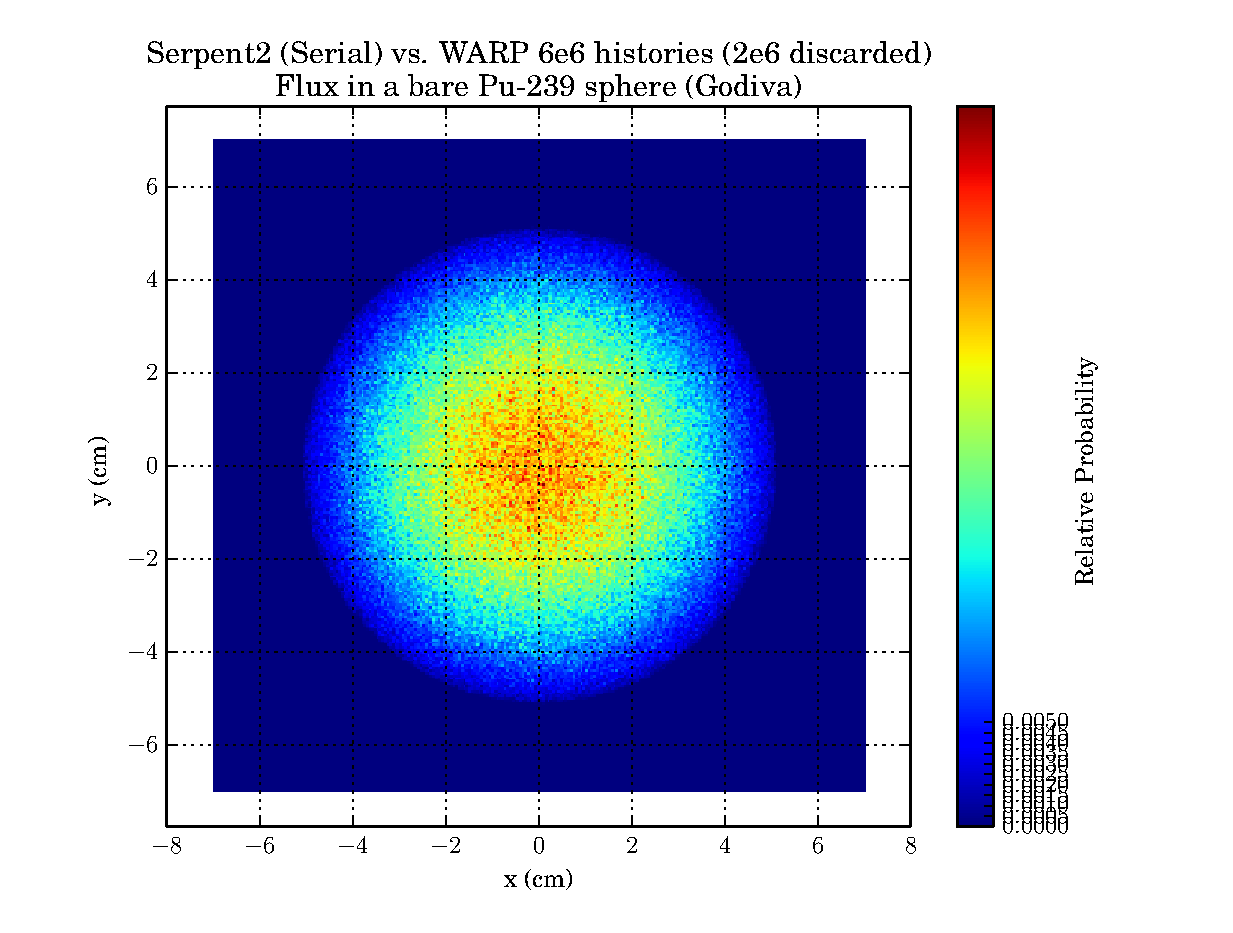
\includegraphics[width=\linewidth]{graphics/finalresults/godiva_fiss2.eps}
  \caption{$x-z$ slice, $y$ collapsed}
  \label{fig:sub2}
\end{subfigure}
\caption{Fission source distribution of a ``godiva'' bare pu-239 sphere. \label{godiva_fiss} }
\end{figure}

\begin{figure}[h!] 
\centering
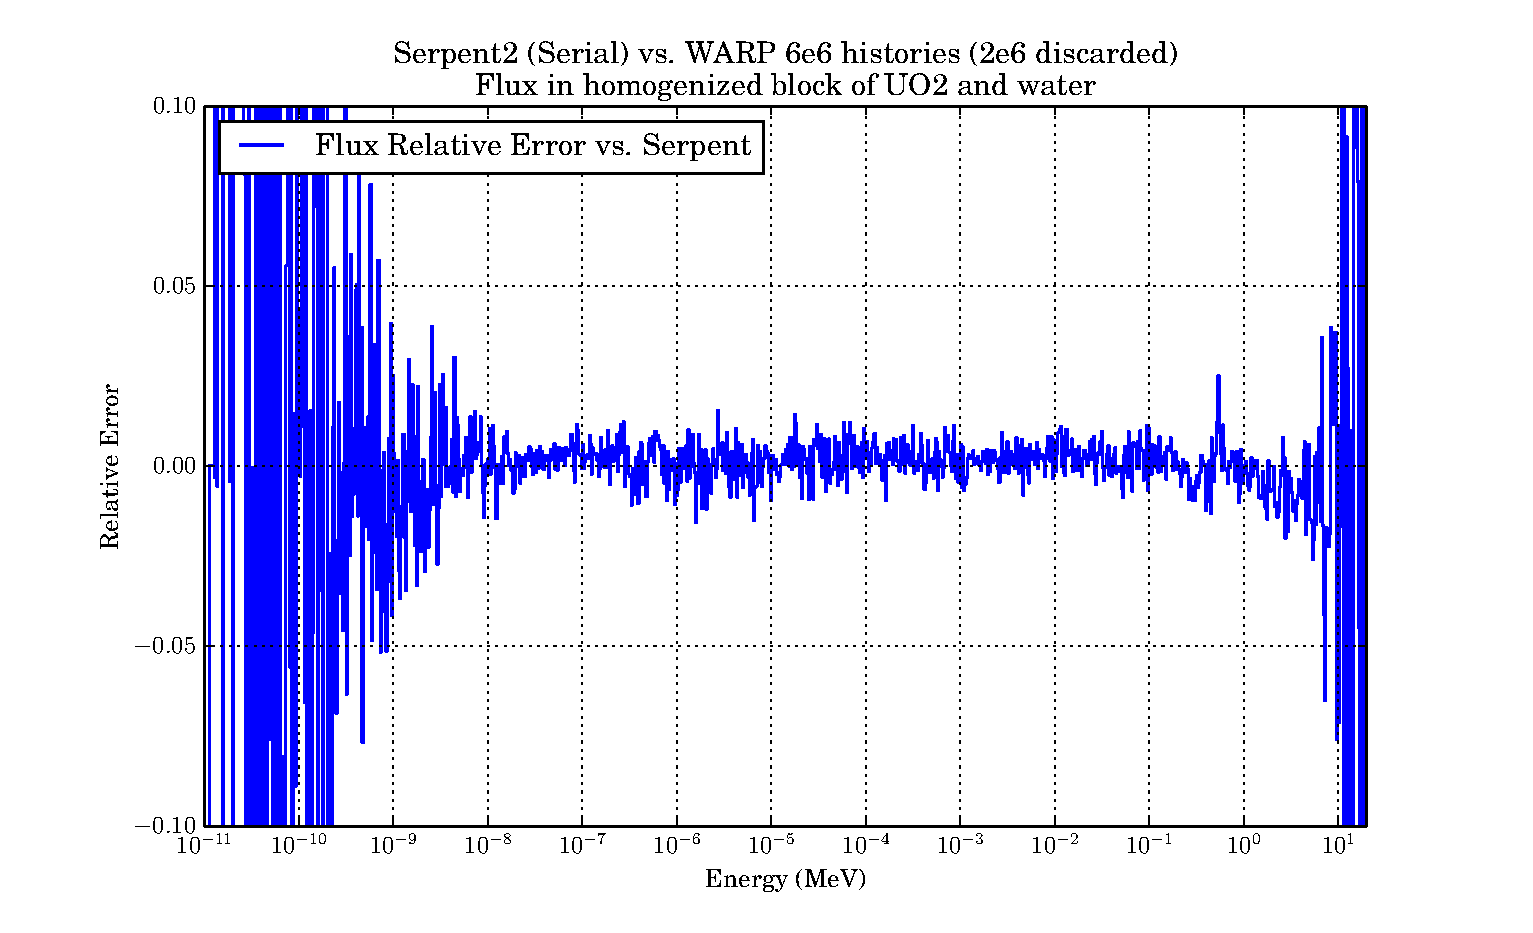
\includegraphics[width=0.8\textwidth]{graphics/finalresults/homfuel_spec_err.eps}
\caption{Error of the spectrum calculated by WARP relative to that of Serpent in a homogenized block of UO$_2$ and water. \label{homfuel_spec_err} }
\end{figure}

\begin{figure}[h!] 
\centering
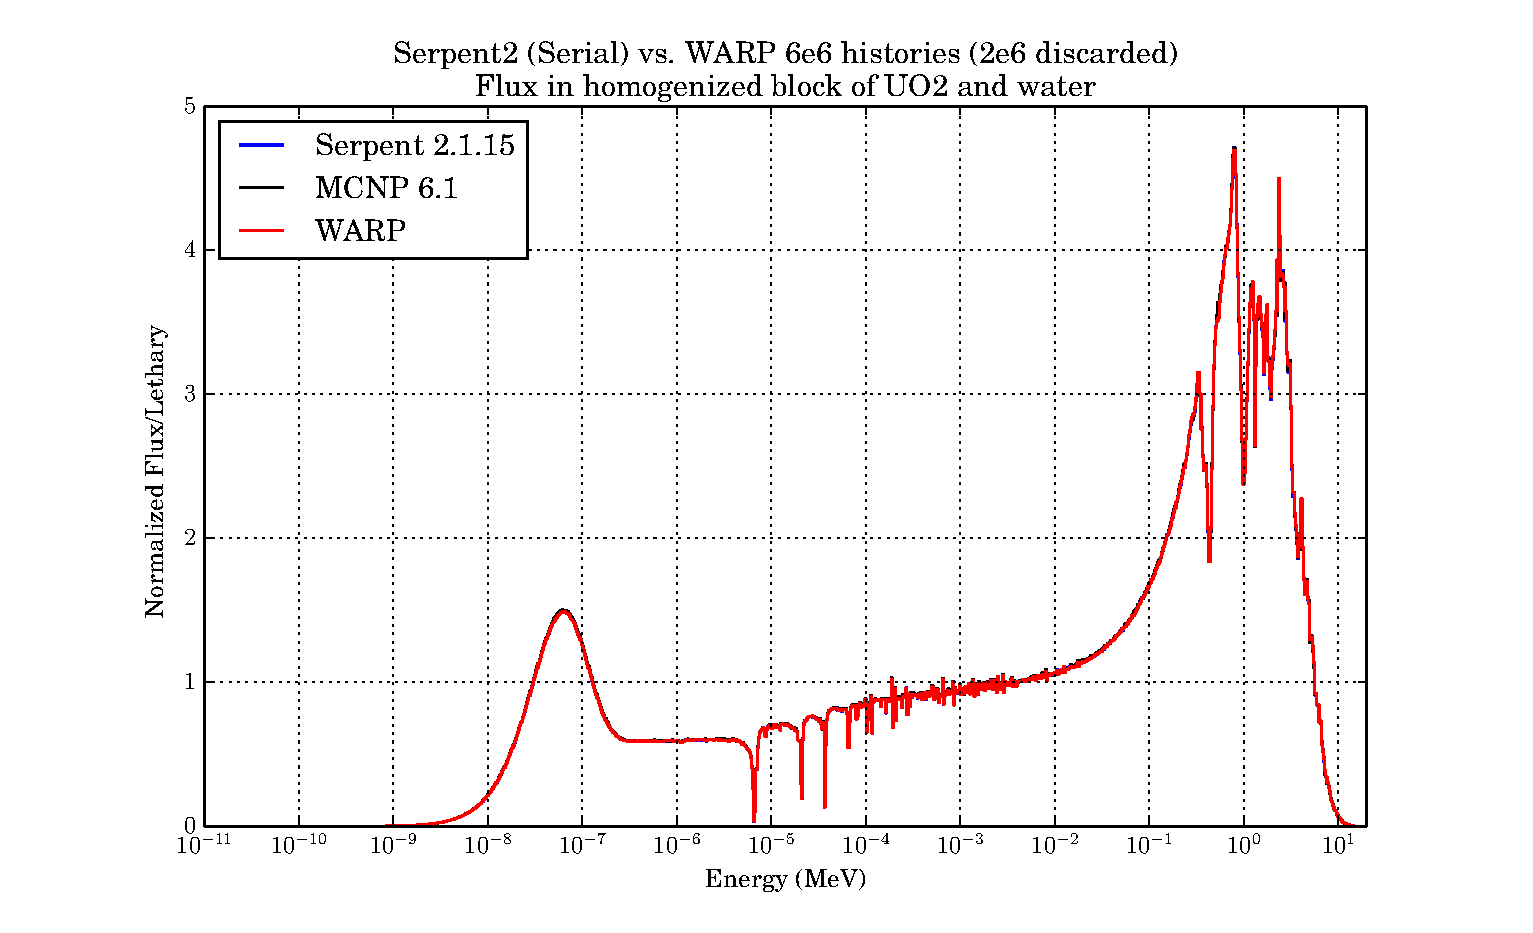
\includegraphics[width=0.8\textwidth]{graphics/finalresults/homfuel_spec.eps}
\caption{Spectrum comparison in a homogenized block of UO$_2$ and water. \label{homfuel_spec} }
\end{figure}

\begin{figure}[h!]
\centering
\begin{subfigure}{.5\textwidth}
  \centering
  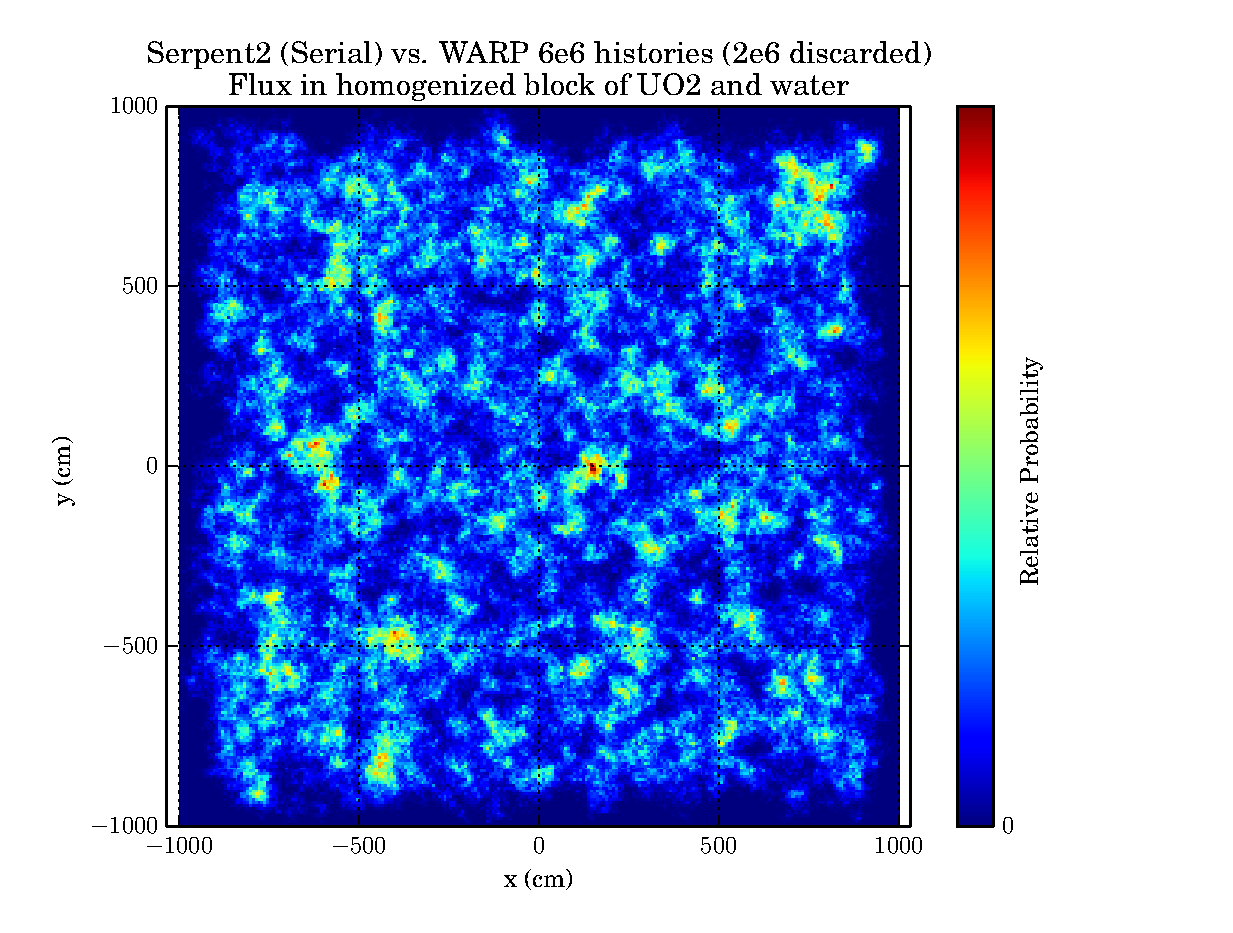
\includegraphics[width=\linewidth]{graphics/finalresults/homfuel_fiss1.eps}
  \caption{$x-y$ slice, $z$ collapsed}
  \label{fig:sub1}
\end{subfigure}%
\begin{subfigure}{.5\textwidth}
  \centering
  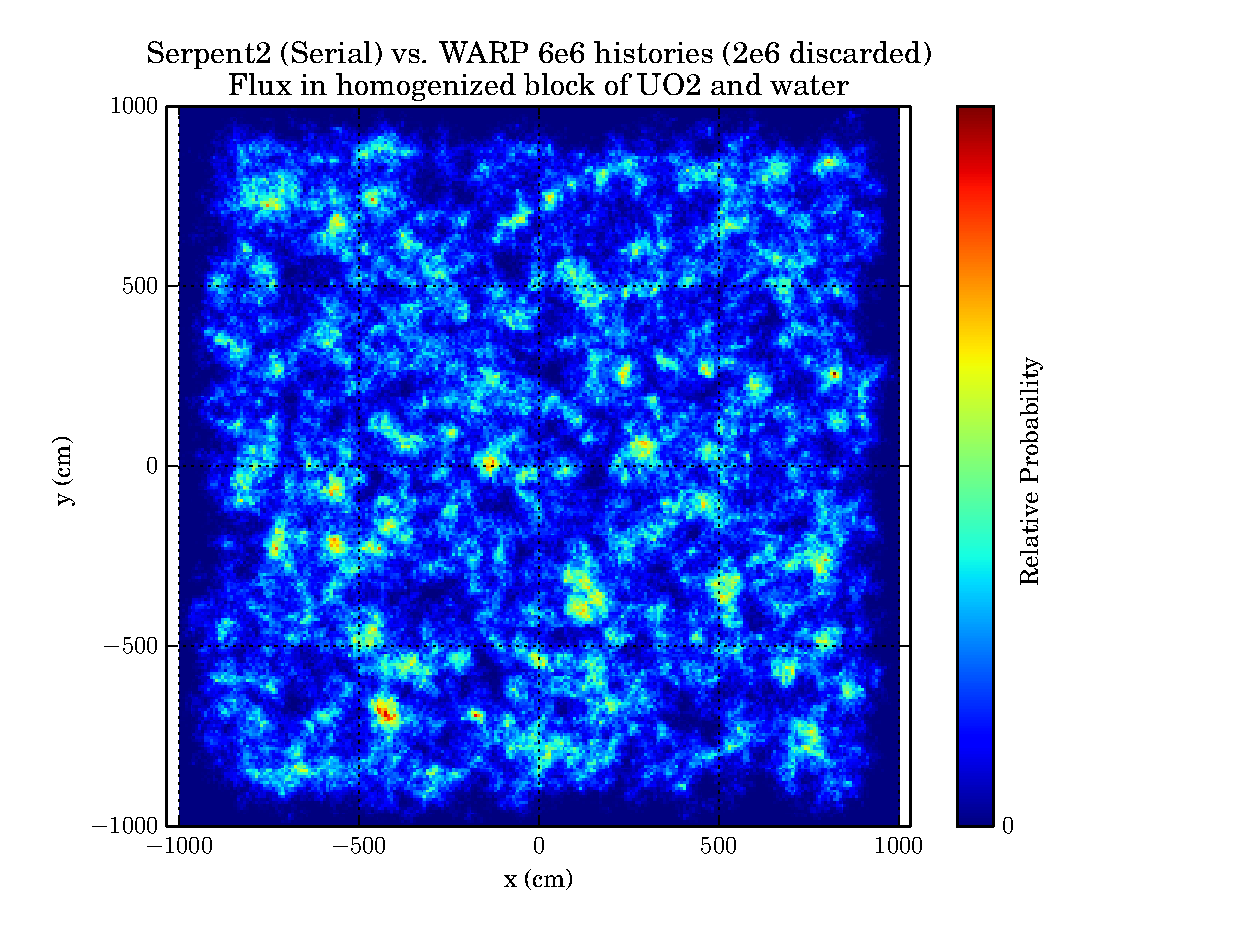
\includegraphics[width=\linewidth]{graphics/finalresults/homfuel_fiss2.eps}
  \caption{$x-z$ slice, $y$ collapsed}
  \label{fig:sub2}
\end{subfigure}
\caption{Fission source distribution of a homogenized block of UO$_2$ and water. \label{homfuel_fiss} }
\end{figure}

\begin{figure}[h!] 
\centering
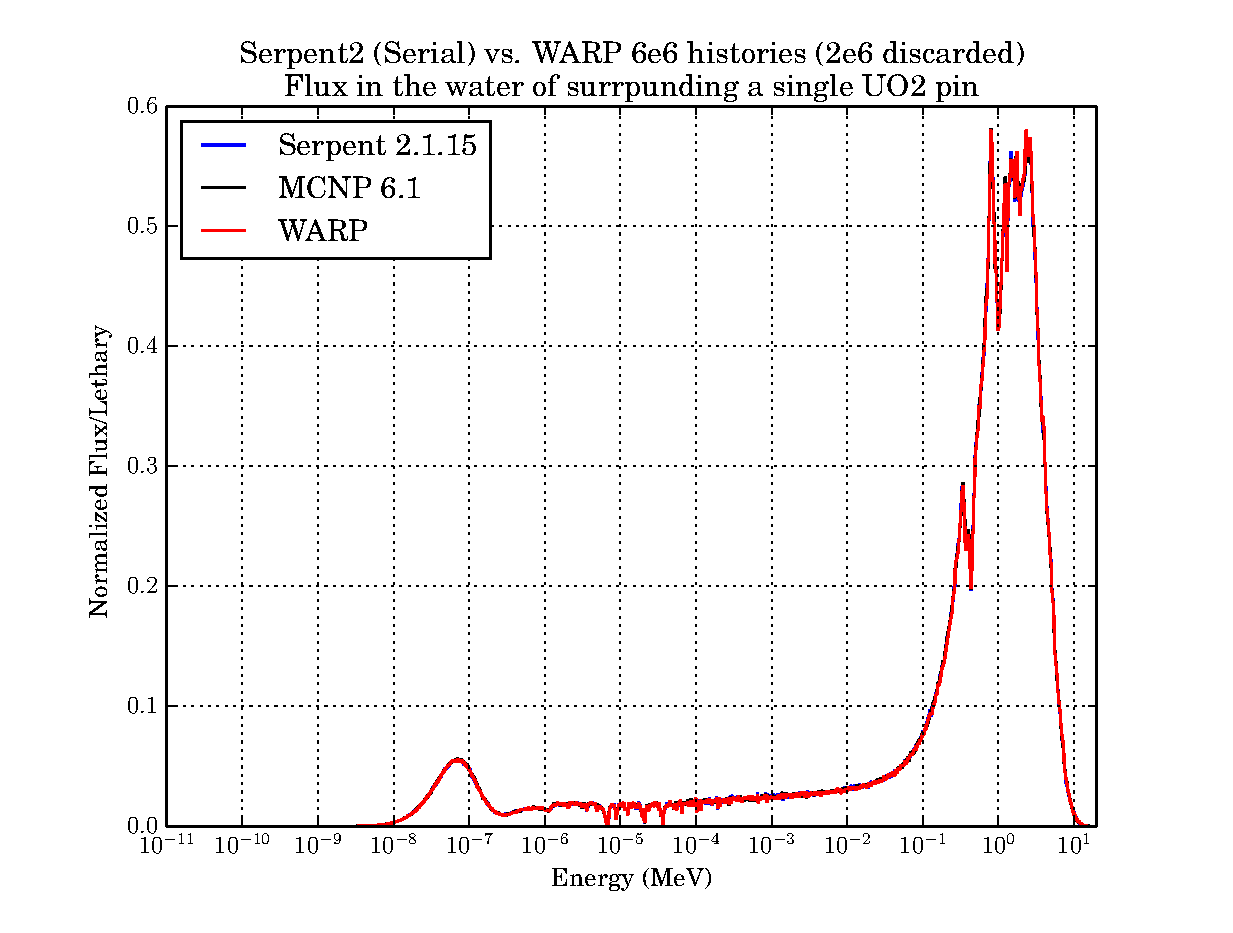
\includegraphics[width=0.8\textwidth]{graphics/finalresults/pincell_spec.eps}
\caption{Spectrum comparison in a single UO$_2$ pin surrounded by a block of water. \label{pincell_spec} }
\end{figure}

\begin{figure}[h!] 
\centering
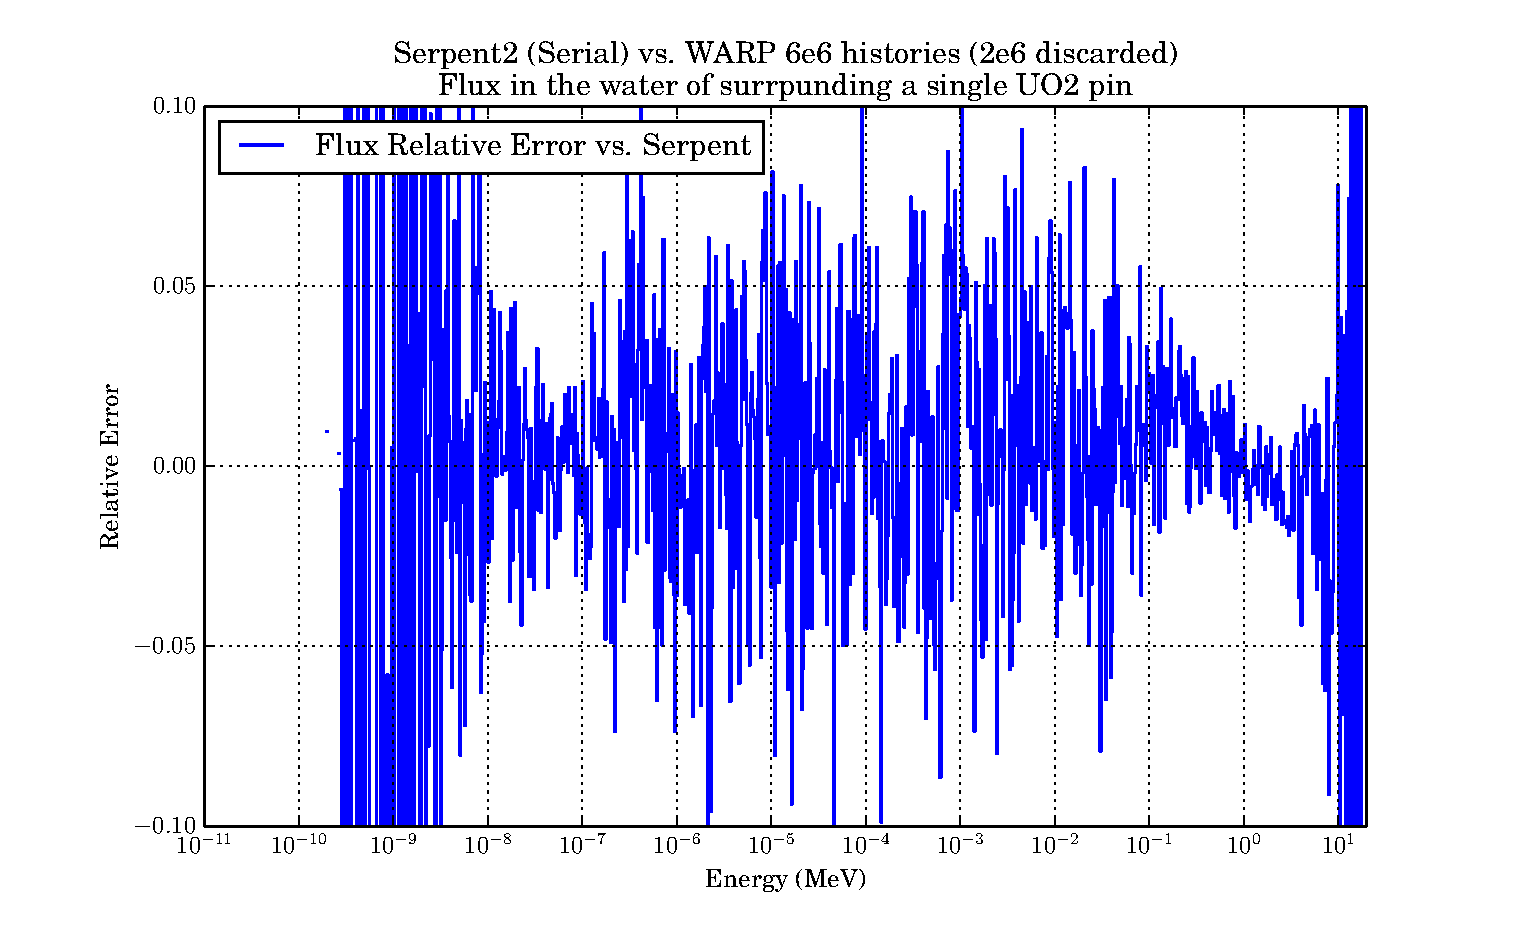
\includegraphics[width=0.8\textwidth]{graphics/finalresults/pincell_spec_err.eps}
\caption{Error of the spectrum calculated by WARP relative to that of Serpent in a single UO$_2$ pin surrounded by a block of water. \label{pincell_spec_err} }
\end{figure}

\begin{figure}[h!]
\centering
\begin{subfigure}{.5\textwidth}
  \centering
  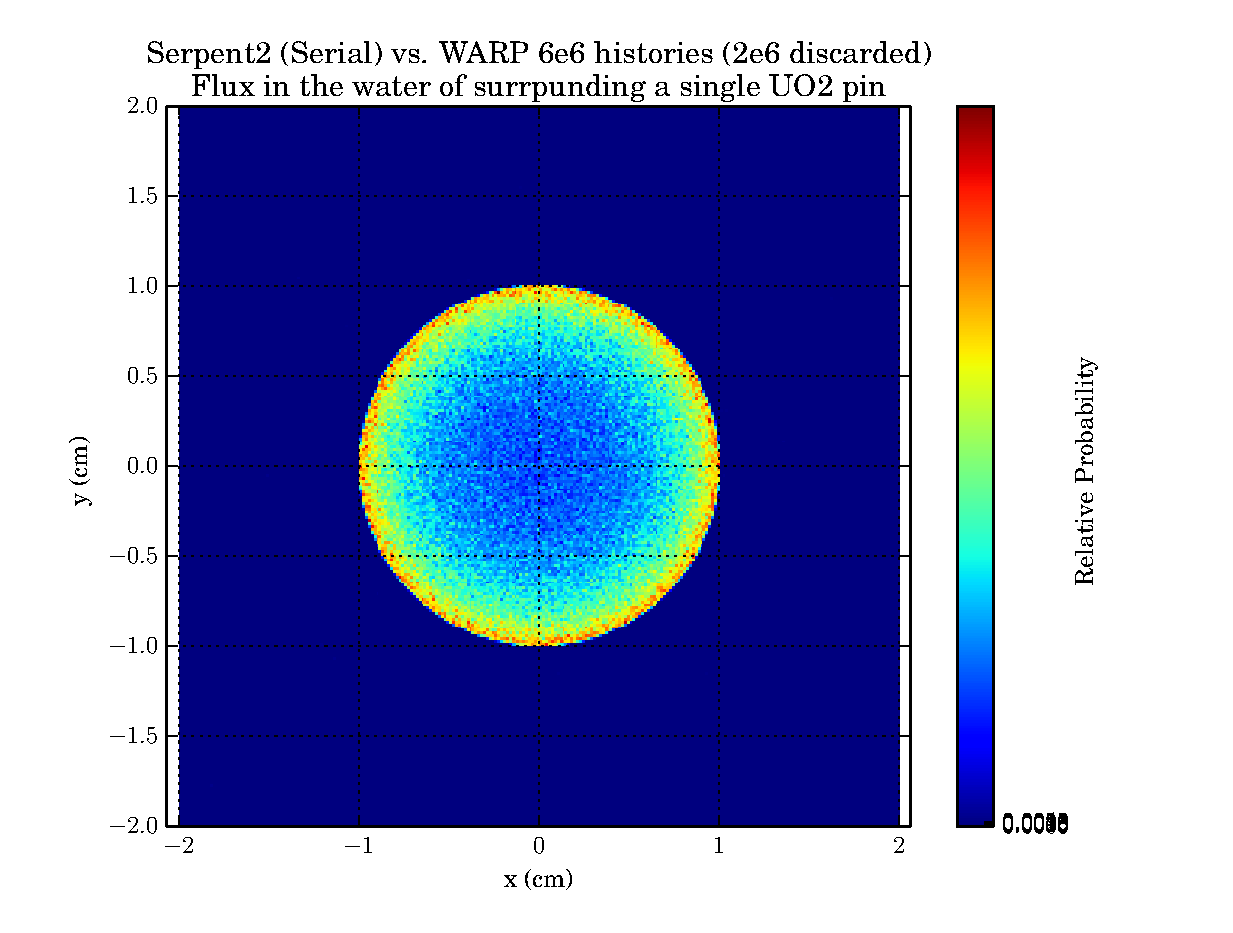
\includegraphics[width=\linewidth]{graphics/finalresults/pincell_fiss1.eps}
  \caption{$x-y$ slice, $z$ collapsed}
  \label{fig:sub1}
\end{subfigure}%
\begin{subfigure}{.5\textwidth}
  \centering
  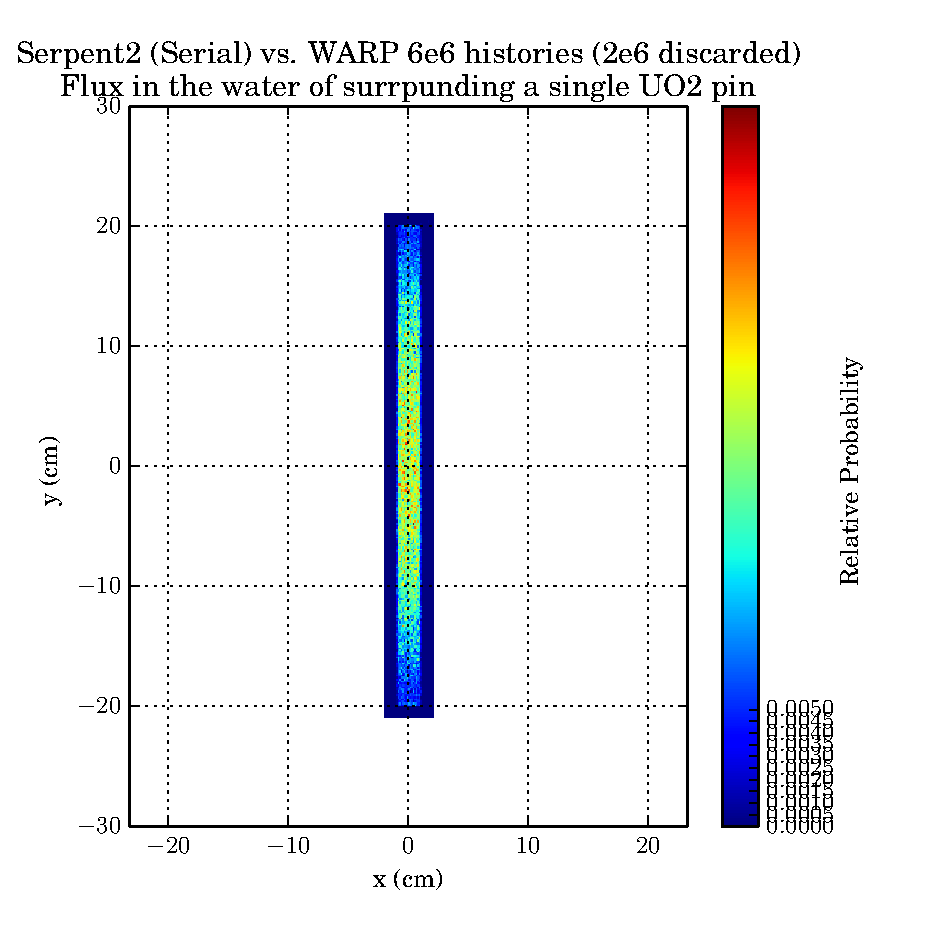
\includegraphics[width=\linewidth]{graphics/finalresults/pincell_fiss2.eps}
  \caption{$x-z$ slice, $y$ collapsed}
  \label{fig:sub2}
\end{subfigure}
\caption{Fission source distribution of a single UO$_2$ pin surrounded by a block of water. \label{pincell_fiss} }
\end{figure}

\begin{figure}[h!] 
\centering
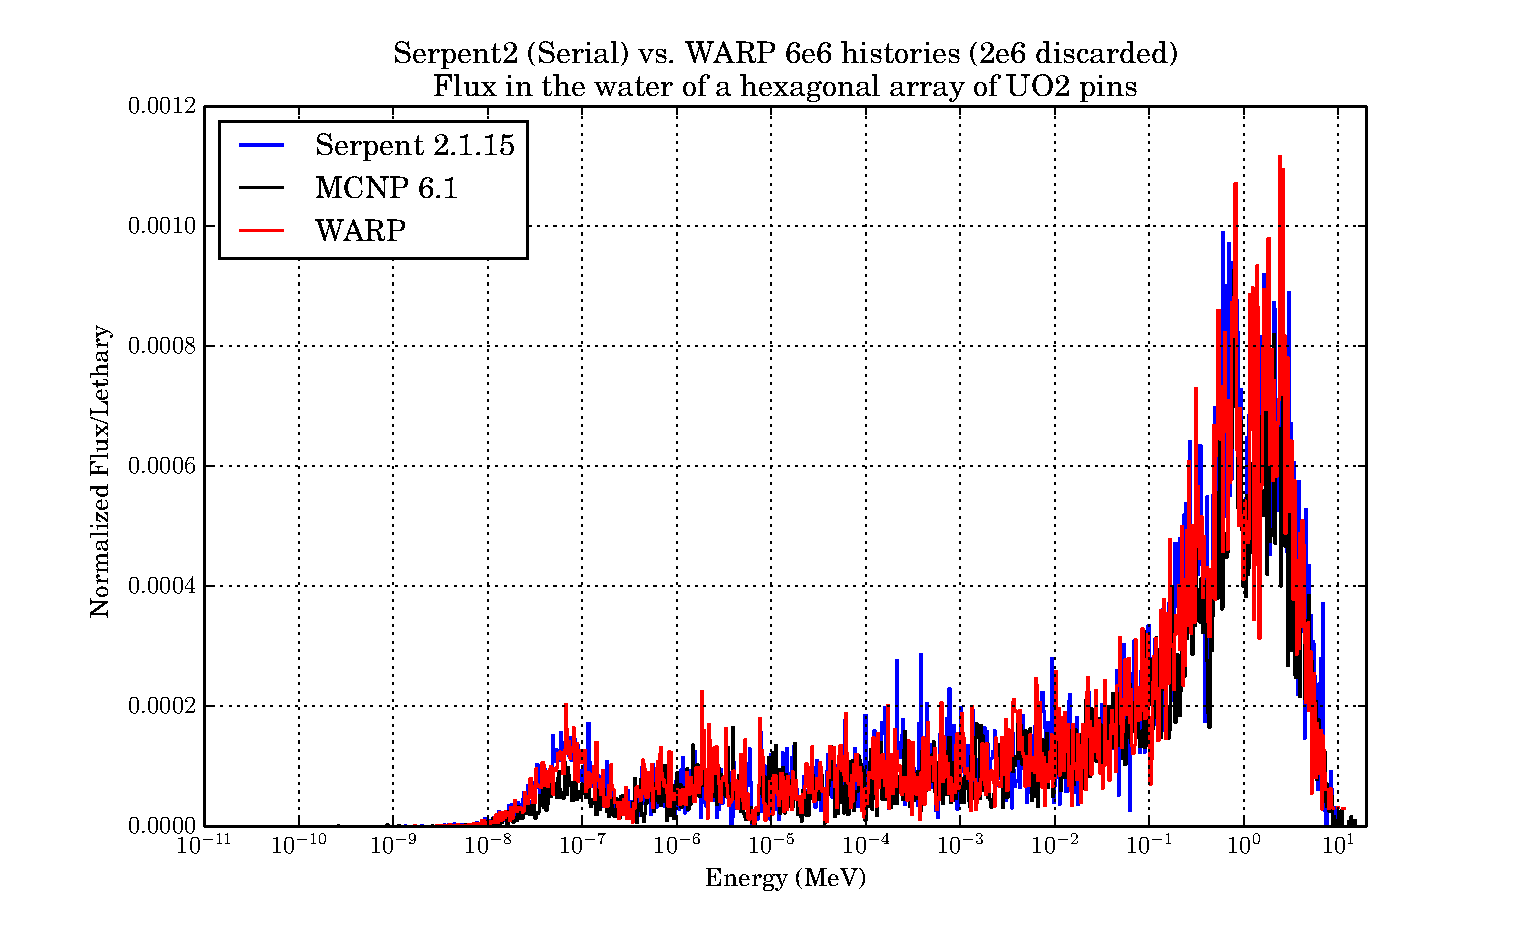
\includegraphics[width=0.8\textwidth]{graphics/finalresults/assembly_spec.eps}
\caption{Spectrum comparison in the center UO$_2$ pin of a 15-sided hex pin array in water. \label{assembly_spec} }
\end{figure}

\begin{figure}[h!] 
\centering
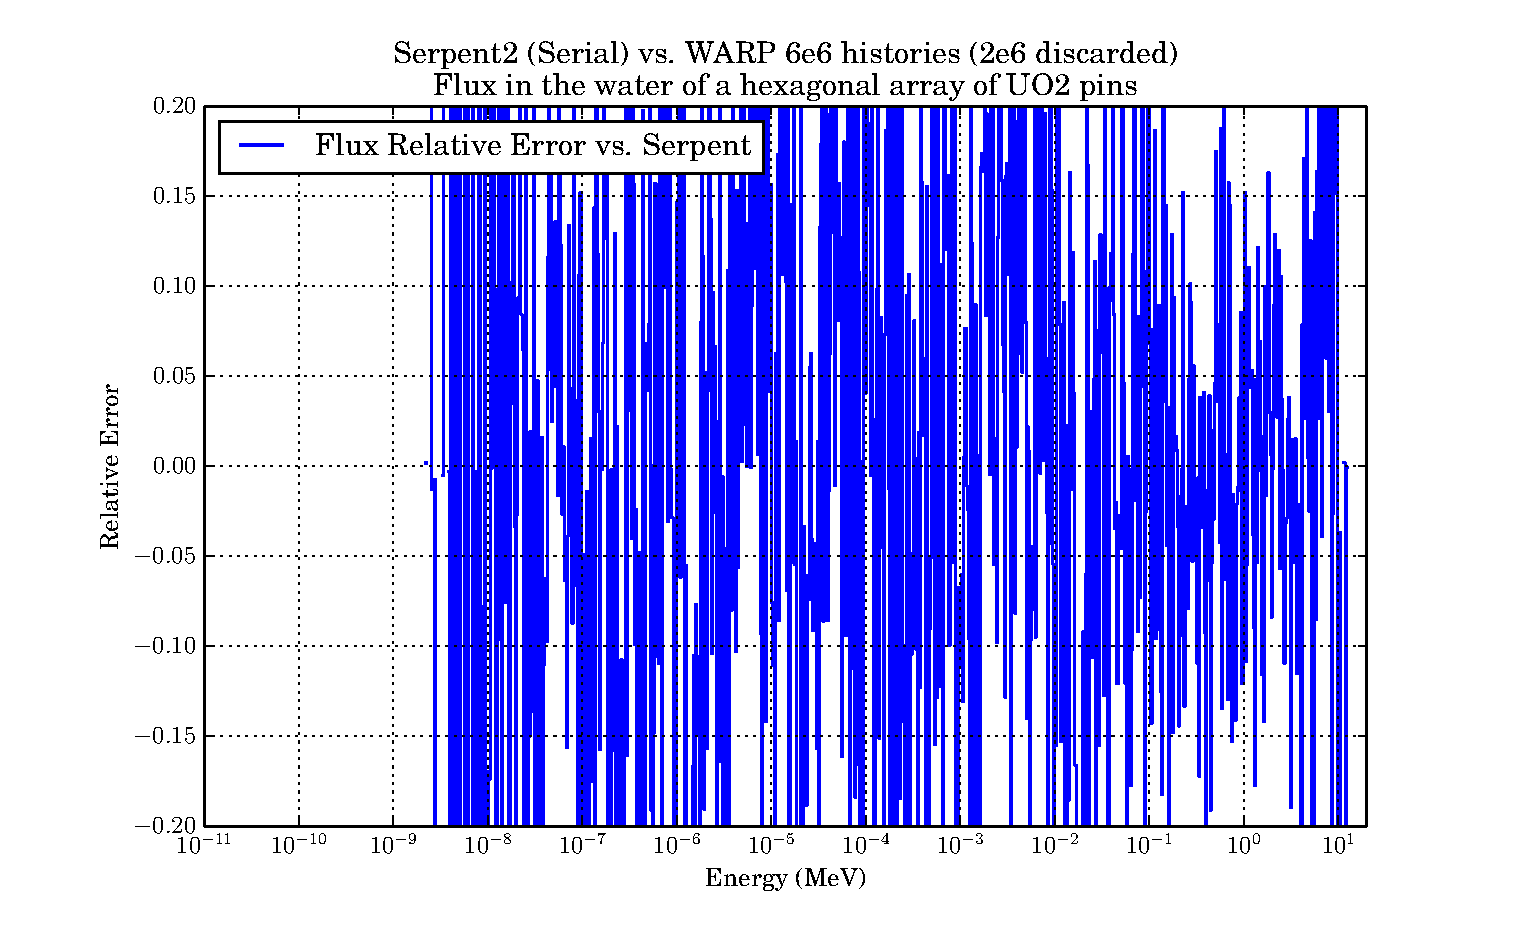
\includegraphics[width=0.8\textwidth]{graphics/finalresults/assembly_spec_err.eps}
\caption{Error of the spectrum calculated by WARP relative to that of Serpent in the center UO$_2$ pin of a 15-sided hex pin array in water. \label{assembly_spec_err} }
\end{figure}

\begin{figure}[h!]
\centering
\begin{subfigure}{.5\textwidth}
  \centering
  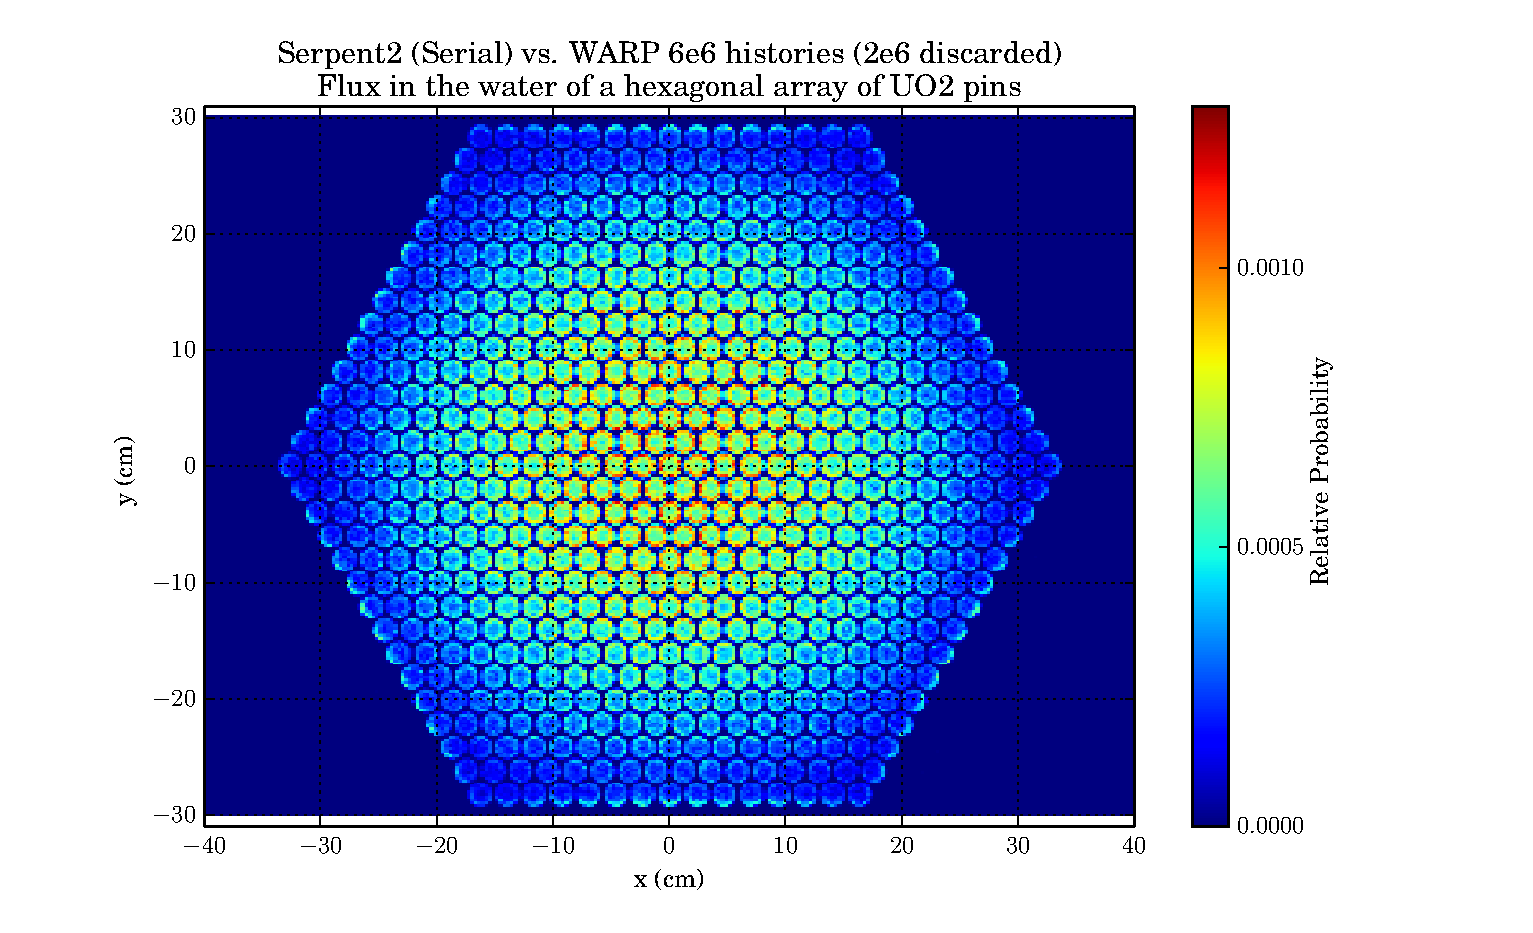
\includegraphics[width=\linewidth]{graphics/finalresults/assembly_fiss1.eps}
  \caption{$x-y$ slice, $z$ collapsed}
  \label{fig:sub1}
\end{subfigure}%
\begin{subfigure}{.5\textwidth}
  \centering
  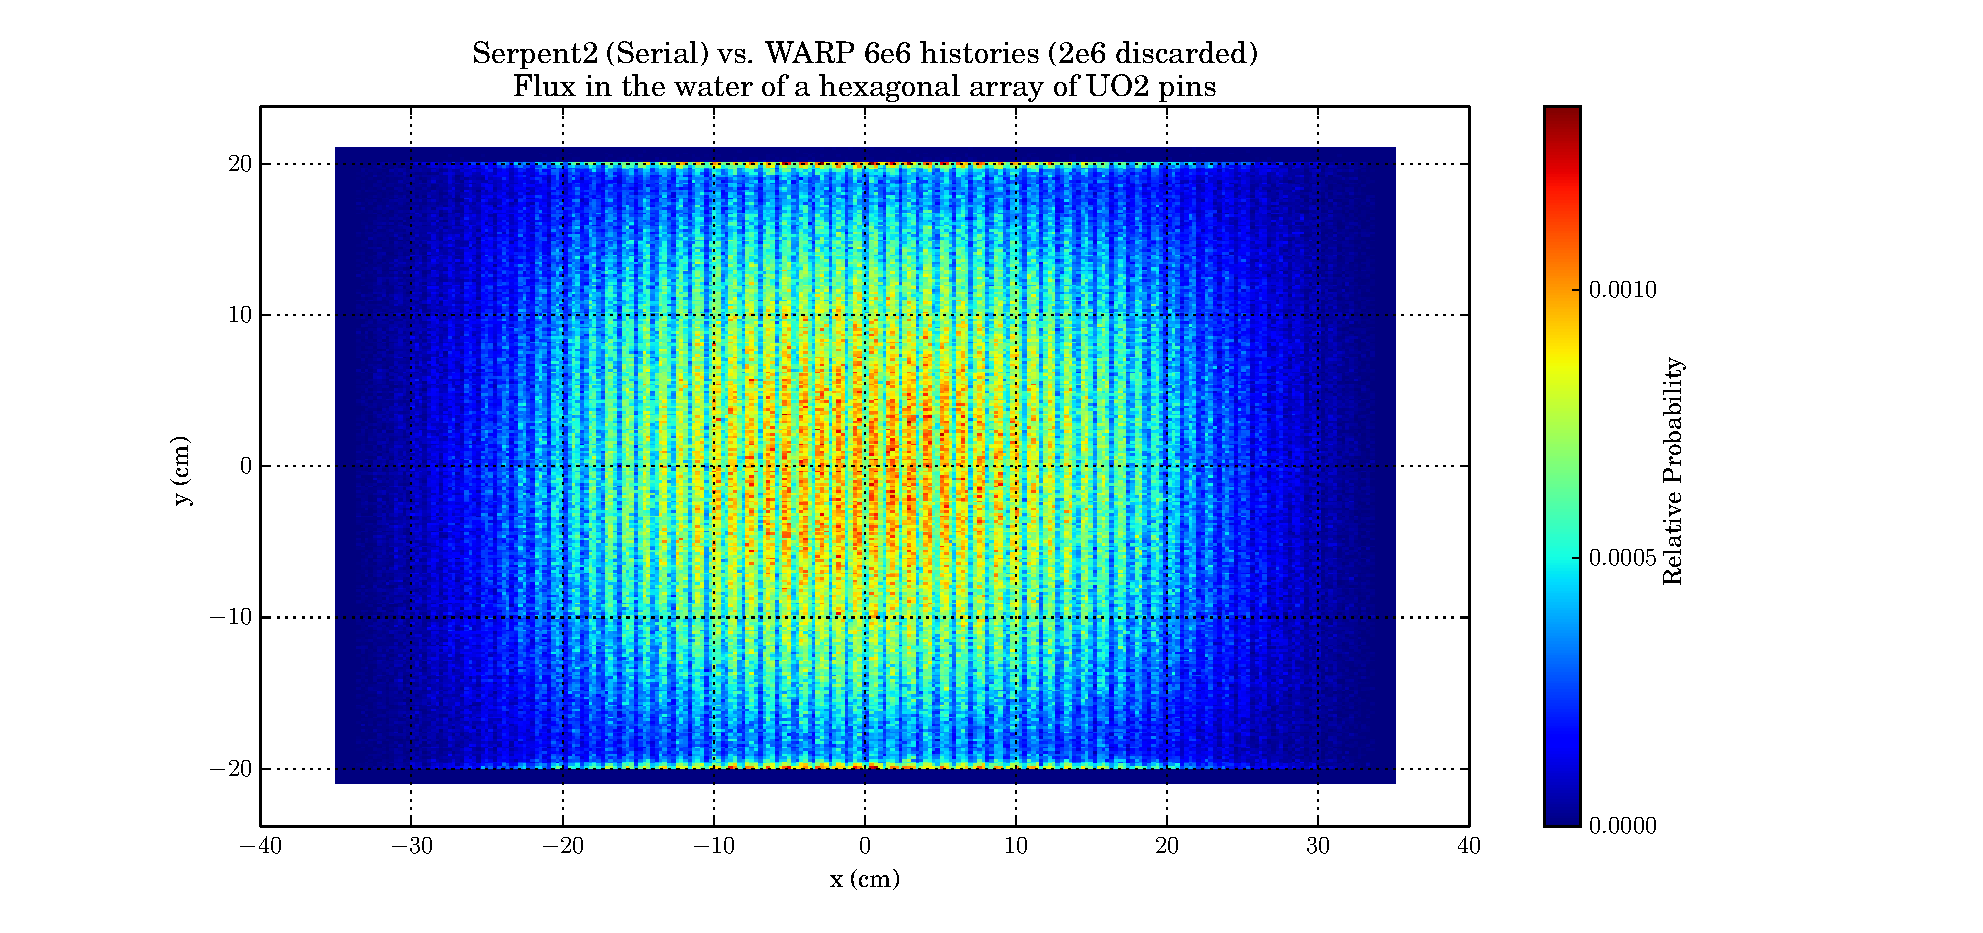
\includegraphics[width=\linewidth]{graphics/finalresults/assembly_fiss2.eps}
  \caption{$x-z$ slice, $y$ collapsed}
  \label{fig:sub2}
\end{subfigure}
\caption{Fission source distribution of an array of UO$_2$ pins in water. \label{assembly_fiss} }
\end{figure}

combine the combo plots into one in python subplots instead of having two large plots.  will then include more color and only one colormap

simple geometry serpent is slow since woodcock makes it sample the geom much more before leaking?, mcnp and warp can instantly leak it?  shouldn't be seen in the homogenized case... yep!


profiler stuff

